\chapter{Lab 4: LQR Optimization for Feedback Control and Observer Design for the Rotary Flexible Beam}

The purpose of this lab is to design and optimize a feedback controller for the rotary flexible beam system. One way of achieving this is to use a Linear Quadratic Regulator, which automates the process of finding a state feedback gain $K$ in a way that optimizes the system for certain design parameters. The prelab focuses on analyzing the stability of the open-loop rotary flexible beam system. In the lab, you will first design and optimize the closed-loop state feedback system by using the LQR technique to minimize the flexible beam's deflections while the rotor base tracks an input signal trajectory. The closed-loop system will have to adhere to set restrictions on settling time, percent overshoot and maximal flexible beam deflection. Next, you will observe the effects of using only partial state feedback on the system response to an input. Finally, you will attempt to minimize these system response effects by building an observer for the unobservable state and using the ensuing state estimate as feedback.
\begin{figure}[htb!]
    \centering
    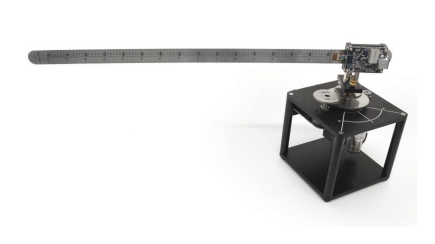
\includegraphics[width=.6\linewidth]{eps/lab_1/quanser.eps}
    \caption{Qanser SRV02 with flexible beam module~\cite{Q-Flex-Beam}.}
    \label{fig:lab4_plant}
\end{figure}

\section{Key Concepts}
\subsubsection{Setting up the Rotary Flexible Beam}\label{sub subsection:lab1_setup}
First, you must assemble and wire the physical system correctly. Examine the close-up assembly shown in Figure~\ref{fig:lab1_assembly} and replicate this at your workstation. Note that the high-gear configuration is used here: a large gear is connected to a small pinion and a slip gear, rather than using the smaller gear. You will need to build a two-tiered gear train as shown in Figure~\ref{fig:lab1_assembly} to make the large gear fit correctly. Use the wiring diagram shown in Figure~\ref{fig:lab1_wiring} to connect the rotary pendulum to a power source and the data acquisition board.
\begin{figure}[htb!]
    \centering
    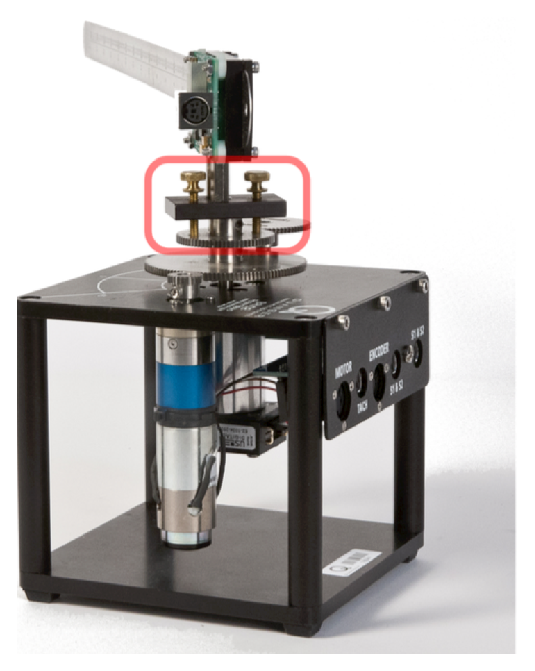
\includegraphics[width=.3\linewidth]{eps/lab_1/assembly.eps}
    \caption{A close-up of the assembly of the rotary flexible beam module and the Quanser SRV02 plant~\cite{Q-Flex-Beam}. The high-gear gear train is indicated by a red box.}
    \label{fig:lab1_assembly}
\end{figure}
\begin{figure}[htb!]
    \centering
    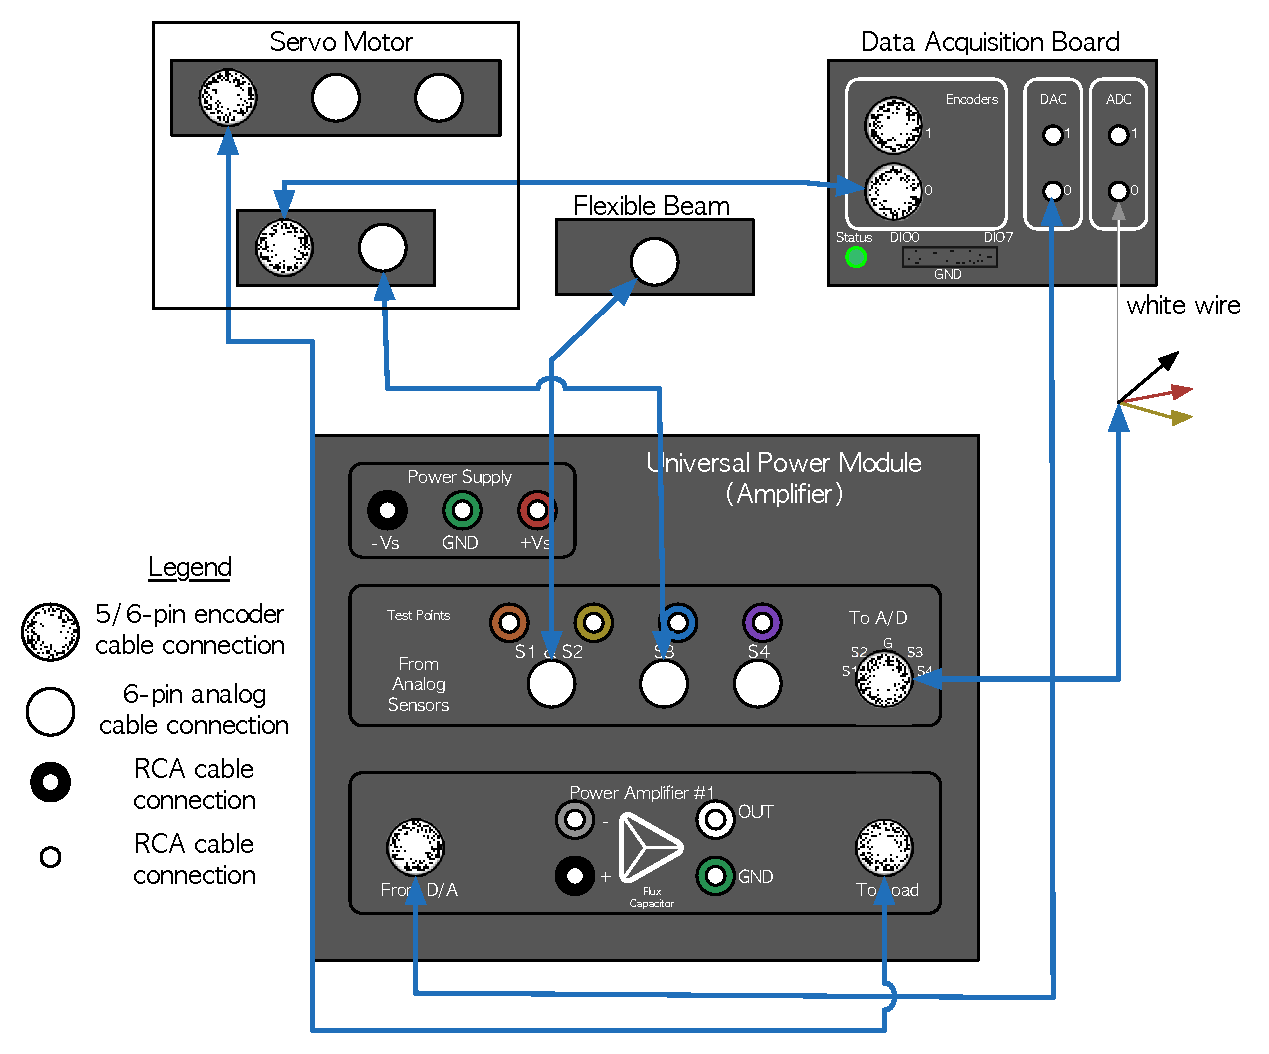
\includegraphics[width=.8\linewidth]{eps/lab_1/wiring.eps}
    \caption{A wiring diagram for the Quanser SRV02 and rotary flexible beam module.}
    \label{fig:lab1_wiring}
\end{figure}

\subsection{The LQ Problem}
A fundamental problem in control theory is operating a control system at minimum cost. When concerned with linear differential equations (e.g., $\mathbf{\dot{x}}(t) = A\mathbf{x}(t) + Bu(t)$) and quadratic cost functions, then one is really concerned with the \emph{LQ problem}. In this lab, we will use a main result from this area of literature~\cite{kwakernaak1972linear} which is the solution to the linear quadratic regulator (LQR). The solution to the LQR will help you design a feedback controller which minimizes the deflections of the flexible beam while the rotor base tracks a square wave trajectory (within certain \emph{design constraints} on settling time and overshoot).

The LQ problem that we are dealing with is an infinite-horizon problem that studies the control system
\[
    \begin{cases}
        \dot{\mathbf{x}}(t) = A\mathbf{x}(t)+Bu(t), \quad \text{where} \; \mathbf{x}(0) = \mathbf{x}_0 \\
        \mathbf{y}(t) = C \mathbf{x}(t)
    \end{cases}
\]
subject to minimizing the cost function
\[
    \eta(u) = \int_0^{\infty} \mathbf{y}^T(t)\mathbf{y}(t) + u^T(t)u(t) \; dt = \int_0^\infty  \mathbf{x}^T(t) C^T C \mathbf{x}(t) + u^T(t)u(t) \; dt.
\]
You may think of the first part of the cost function, $ \int_0^{\infty} \mathbf{y}^T(t)\mathbf{y}(t) dt$, as the \emph{energy of the controlled output}, and the second part, $\int_0^{\infty} u^T(t)u(t) dt$, as the \emph{energy of the control input}.

Two \textbf{main results} from class follow this reformulation: the first is that if $(A,B,C)$ is a minimal realization, then there exists a positive definite symmetric solution $\Pi_{\infty} \in \mathcal{M}^{n \times n}(\mathbb{R})$ to the continuous algebraic Ricatti equation (CARE):
\[
    A^T \Pi_{\infty} + \Pi_{\infty} A - \Pi_{\infty} B B^T \Pi_{\infty} = -C^T C;
\]
the next main result is that with $(A,B,C)$ a minimal realization, the controller
\[
    u(t) = -B^T \Pi_{\infty} \mathbf{x}(t)
\]
solves the LQ problem.

\section{Background Information}\label{section:lab4_prelab}
The following sections will provide relevant matrices/equations for the lab. Don't get too caught up in the calculations, just understand the rough ideas, and use the provided matrices/equations as required.

\subsection{Equations of Motion for the Rotary Flexible Beam}
In a similar fashion to Lab 3, one can find the EOMs for the rotary flexible beam using the Euler-Lagrange equation. The necessary equations are:

\begin{equation*}
    \begin{cases}
        T = \frac{1}{2}J_r \dot{\theta}^2 + \frac{1}{2} J_b \left(\dot{\theta}+\dot{\alpha}\right)^2 \\
        V = \frac{1}{2} K_b \alpha^2
    \end{cases}
\end{equation*}

\[
    \begin{cases}
        \frac{\partial L}{\partial \theta}=0                                                                                             \\
        \frac{\partial L}{\partial \dot{\theta}}=J_r\dot{\theta}+J_b\left(\dot{\theta}+\dot{\alpha}\right)                               \\
        \frac{d}{dt} \left(\partial \frac{L}{\partial \dot{\theta}}\right)= J_r\ddot{\theta}+J_b\left(\ddot{\theta}+\ddot{\alpha}\right) \\
    \end{cases}
\]

\[
    \begin{cases}
        \frac{\partial L}{\partial \alpha}=K_b\alpha                                                                    \\
        \frac{\partial L}{\partial \dot{\theta}}=J_b\left(\dot{\theta}+\dot{\alpha}\right)                              \\
        \frac{d}{dt} \left(\frac{\partial L}{\partial \dot{\theta}}\right)= J_b\left(\ddot{\theta}+\ddot{\alpha}\right) \\
    \end{cases}
\]

which yield, via the Euler-Lagrange equation,

\[
    \left(J_r + J_b\right)\ddot{\theta} + J_b \ddot{\alpha} = \tau - B_r \dot{\theta}.
\]

\[
    J_b \left(\ddot{\theta} + \ddot{\alpha}\right) + K_b \alpha = -B_b \dot{\alpha}.
\]

Thus, letting our state be
\[
    x(t) =
    \left[\begin{array}{c}
            \theta(t)       \\
            \alpha(t)       \\
            \dot{\theta}(t) \\
            \dot{\alpha}(t)
        \end{array}\right].
\]
and assuming the viscous damping of the beam is negligible (so $B_b = 0$), we get the following state-space representation:

\[
    \left[\begin{array}{c}
            \dot{\theta}(t)  \\
            \dot{\alpha}(t)  \\
            \ddot{\theta}(t) \\
            \ddot{\alpha}(t)
        \end{array}\right] =
    \left[\begin{array}{c c c c}
            0 & 0                                          & 1                & 0 \\
            0 & 0                                          & 0                & 1 \\
            0 & \frac{K_b}{J_r}                            & -\frac{B_r}{J_r} & 0 \\
            0 & -\frac{K_b\left(J_b + J_r\right)}{J_b J_r} & \frac{B_r}{J_r}  & 0
        \end{array}\right]
    \left[\begin{array}{c}
            \theta(t)       \\
            \alpha(t)       \\
            \dot{\theta}(t) \\
            \dot{\alpha}(t)
        \end{array}\right] \\ +
    \left[\begin{array}{c}
            0             \\
            0             \\
            \frac{1}{J_r} \\
            -\frac{1}{J_r}
        \end{array}\right] \tau
\]

Evaluating these matrices numerically, we get

\[
    A =
    \left[\begin{array}{c c c c}
            0 & 0       & 1      & 0 \\
            0 & 0       & 0      & 1 \\
            0 & 623.77  & -40.49 & 0 \\
            0 & -965.53 & 40.49  & 0
        \end{array}\right]
\]
and
\[
    B =
    \left[\begin{array}{c}
            0      \\
            0      \\
            61.775 \\
            -61.775
        \end{array}\right].
\]

And using the fact that \(y = Cx + Du\),

\[
    C =
    \left[\begin{array}{c c c c}
            1 & 0 & 0 & 0 \\
            0 & 1 & 0 & 0
        \end{array}\right]
\]
and
\[
    D =
    \left[\begin{array}{c}
            0 \\
            0
        \end{array}\right],
\]

We note that the open-loop poles (that is, the eigenvalues of \(A\)) are $\{0,\; -8.13+22.47i,\; -8.13-22.47i,\; -24.21\}$, and both the algebraic and geometric multiplicities are equal, thus the system is internally stable.

To verify whether we can use full state feedback to steer the system, one must compute the controllability matrix:
\[
    \mathcal{C}_{(A,B)} = \left[\begin{array}{c c c c}
            0      & 61.77    & -2501.26  & 62750.59   \\
            0      & -61.77   & 2501.26   & -41639.42  \\
            61.77  & -2501.26 & 62750.59  & -980692.86 \\
            -61.77 & 2501.26  & -41639.42 & 125861.00
        \end{array}\right]
\]
The system's controllability matrix has full rank, and hence the system is controllable. Thus, we can hope to use full state feedback and pole placement techniques to control the system.

\section{Procedure}
\begin{enumerate}

    \item \textbf{Designing Feedback using the Linear Quadratic Regulator}\label{section:lab4_lqr}

          \begin{enumerate}
              \item What does it mean to be a minimal realization? Is the state-space model of the rotary flexible beam system a minimal realization? Can one hope to use the LQR approach to optimize the feedback control inputs for the rotary flexible beam system?

                    %\drew{Answer: Given any transfer function, any state-space model that is both controllable and observable and has the same input-output behaviour as the transfer function is said to be a minimal realization. As was shown in Lab 1, the state-space model of the rotary flexible beam accurately describes the physical system; since the transfer function describes the input and output behaviour of the physical system, one can conclude that the state-space model has the same input-output behaviour as the transfer function. Furthermore, the observability matrix for the state-space model is
                    %\[
                    %\mathcal{O}_{(C,A)} = \left[\begin{array}{c c c c}
                    %1 & 0 & 0 & 0\\
                    %0 & 1 & 0 & 0\\
                    %0 & 0 & 1 & 0\\
                    %0 & 0 & 0 & 1\\
                    %0 & 623.77 & -40.49 & 0\\
                    %0 & -965.53 & 40.49 & 0\\
                    %0 & -25257.84 & 1639.61 & 623.77\\
                    %0 & 25257.84 & -1639.61 & -965.53
                    %\end{array}\right]
                    %\]
                    %which has full rank (see prelab for computation of $\mathcal{C}_{(A,B)}$, which also has full rank). Thus, $(A,B,C)$ is a minimal realization, and one can use the main results for LQR theory to optimize the feedback control inputs for the physical system. 
                    %}
                    \vspace{0.5em}
                    There are a few differences in the theory that you've learned from class and the treatment we will apply here. First, we wish to minimize some of the system's outputs more than others, e.g., our focus is on minimizing the flexible beam deflections. With this focus, we present a more generalized form of the quadratic cost function:
                    \begin{equation}\label{lab4_cost_function}
                        \eta(u) = \int_0^{\infty} \mathbf{x}^T(t) Q \mathbf{x}(t) + u^T(t)u(t) \; dt,
                    \end{equation}
                    where $Q$ is symmetric and $\mathbf{x}^T(t) Q \mathbf{x}(t) > 0$ for all $t$ (positive-definite). You will set the matrix $Q$ as a diagonal weighting matrix to assign different weights on the states within the cost function~\eqref{lab4_cost_function}. In turn, this will determine how the control input $u(t)$ will minimize the cost function $\eta(u)$, and thus the weightings of matrix $Q$ will have direct effects on the ensuing feedback gain, $K$. Hence, the LQR design process is really an iterative process: tune the diagonal weightings of $Q$, observe the effects, compare against the desired performance metrics, and repeat.

                    In the theory from class, one had to verify that $(A,B,C)$ was a minimal realization in order for $u(t)=-B^T \Pi_{\infty} \mathbf{x}(t)$ to solve the LQ problem. Using the generalized quadratic cost function in~\eqref{lab4_cost_function}, one must only verify that $(A,B)$ be stabilizable to ensure that this input solves the LQ problem. Can the LQR approach be used to optimize the feedback control inputs for the rotary flexible beam?
                    %\drew{Answer: stabilizability follows from the fact that the system is controllable (see previous answer for $\mathcal{C}_{(A,B)}$ computation).}

                    Open the Simulink model \textbf{lqr\_model.mdl}, shown in Figure~\ref{lab4_lqr_simulink}. Notice the presence of a high-gain observer, used to estimate the time derivatives of the signals $\theta$ and $\alpha$, as was discussed in Section~\ref{section:lab3_feedback} of Lab 3. In this lab, you will use these signal derivative estimates as feedback. Notice also that the output signal is subtracted from the input signal before being scaled by the feedback gain. Thus when the system's outputs match the system's inputs, a signal of all zeros will be input into the physical system; when the system inputs and outputs do not match, the feedback gain should be designed to drive the non-zero states to zero (this will work if $K$ is designed to make the closed-loop system \emph{asymptotically stable}).
                    \begin{figure}[htb!]
                        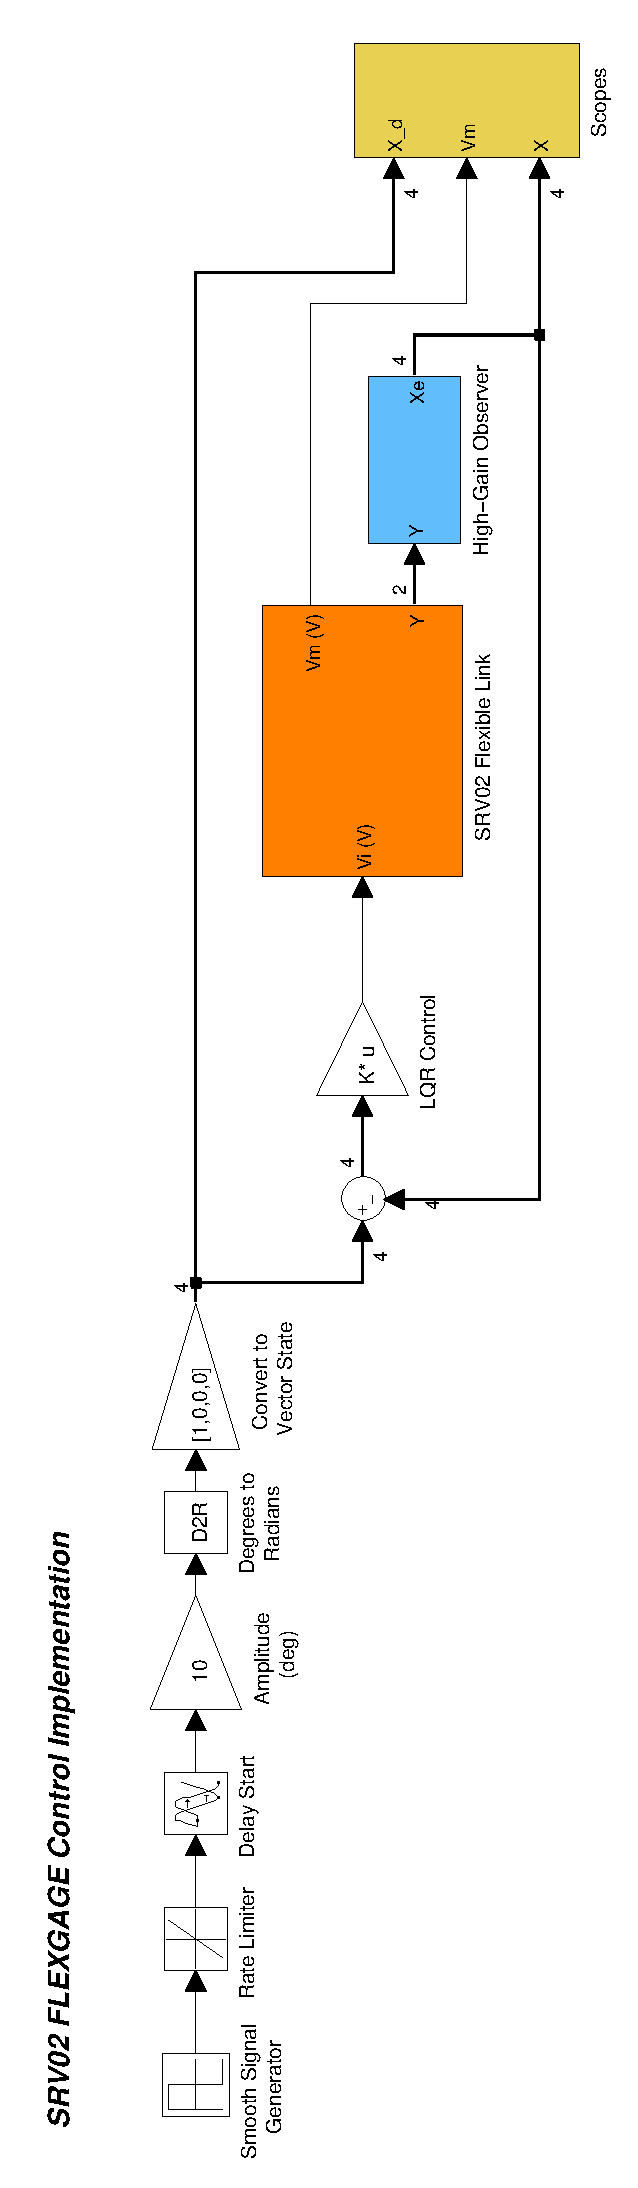
\includegraphics[width=0.3\linewidth,angle=-90]{eps/lab_4/lqr_simulink}
                        \caption{A Simulink model that inputs a signal into the rotary flexible beam system and observes its output. This model can be used to drive the rotor base to track a signal input while minimizing the flexible beam deflections via full state feedback. The feedback gain $K$ is designed using a linear quadratic regulator.}
                        \label{lab4_lqr_simulink}
                    \end{figure}

                    Your first task will be to observe the effects of changing the diagonal weightings of $Q$. Using your state-space matrices from Section~\ref{section:lab4_prelab}, and setting
                    \[
                        Q = \left[\begin{array}{c c c c}
                                q_1 & 0   & 0   & 0   \\
                                0   & q_2 & 0   & 0   \\
                                0   & 0   & q_3 & 0   \\
                                0   & 0   & 0   & q_4
                            \end{array}\right]
                    \]
                    you can use the MATLAB command \emph{care} to solve the continuous algebraic Ricatti equation (CARE). This will return the solutions to the Riccati equation, $\Pi_{\infty}$, which you will use to compute your feedback gain, $K=-B^T \Pi_{\infty}$.
              \item Using a diagonal weightings matrix for $Q$, express the cost function symbolically. What would be the effect of increasing the diagonal elements $q_i$ on the feedback gain, $K$?
                    %\drew{Answer:
                    %\begin{align*}
                    %\eta(u) &= \bigint_0^{\infty} \left( [\theta \quad \alpha \quad \dot{\theta} \quad \dot{\alpha}] \left[\begin{array}{c c c c} 
                    %q_1 & 0 & 0 & 0\\
                    %0 & q_2 & 0 & 0\\
                    %0 & 0 & q_3 & 0\\
                    %0 & 0 & 0 & q_4
                    %\end{array}\right] \left[\begin{array}{c} \theta \\ \alpha \\ \dot{\theta} \\ \dot{\alpha} \end{array}\right] + u^T(t)u(t) \right)\; dt \\
                    %& = \int_0^{\infty} q_1\theta^2 + q_2\alpha^2 + q_3\dot{\theta}^2 + q_4\dot{\alpha}^2 +u^2(t) \; dt
                    %\end{align*}
                    %Increasing the weightings $q_i$ would alter the cost function so as to give the corresponding state more influence over the cost, e.g., increasing $q_1$ would cause the control input $u(t)$ to have a bias towards minimizing the state scaled by $q_1$ (in our lab, this state is $\theta$), and thus would increase the corresponding feedback gain element $k_1$ to compensate, where
                    %\[
                    %K = \left[\begin{array}{c} k_1 \\ k_2 \\ k_3 \\ k_4 \end{array}\right].
                    %\]
                    %This behaviour is the same for all weightings $q_i$. Note that due to the interconnectedness of the system states, changing one $q_i$ may (and usually will) effect multiple states.
                    %}
              \item \emph{Check your feedback gain with your TA}. Since the Simulink model \emph{subtracts} the feedback from the input, make sure you define $K$ as $K=B^T \Pi_{\infty}$ and \textbf{not} $-K=B^T \Pi_{\infty}$. Vary the weightings $q_1,\; q_2,\; q_3,\; q_4$ independently from starting values $[q_1,\; q_2,\; q_3,\; q_4] = [1,\; 1,\; 1,\; 1]$. Run \textbf{lqr\_model.mdl} with a square wave input of amplitude 30 \textbf{total} (there is a signal amplitude \& an amplitude block, multiply these to get 30) and with frequency of 0.33 Hz. What effects does each modification have on the feedback gain, $K = [k_1,\; k_2,\; k_3,\; k_4]$? Plot each of the state responses with respect to time. What effects does each modification have on the physical system's state responses? What weighting(s) has(have) noticeable effects on reducing the rise time (one in particular is noticeable)? Did any decrease the flexible beam's deflections? \emph{Formulate problems and their specifications} that you anticipate when tuning particular weightings in various \emph{engineering applications} (e.g., for tidal power generators - or flexible beams mounted on the ocean floor in locations of notably strong tidal power - where the flexible beam's deflections trigger a power generator, but can also be strained to failure).
                    %\drew{Answer: Here are the plots and the corresponding feedback gains produced by the linear quadratic regulator:
                    %\begin{figure}[htb!]
                    %\subfigure{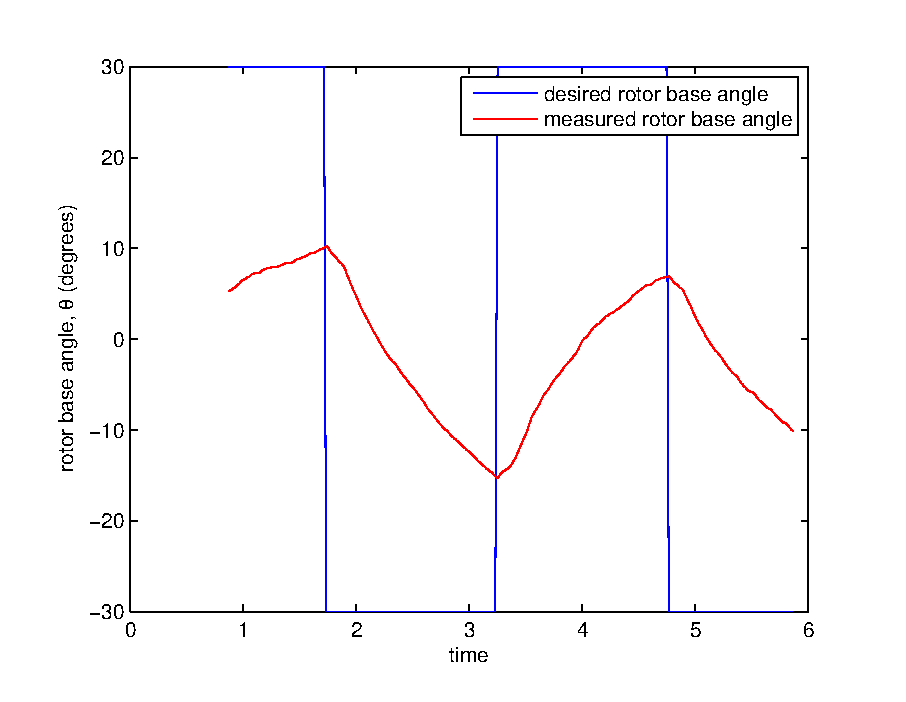
\includegraphics[width=0.5\linewidth]{eps/lab_4/theta_q_1_1_1_1}}
                    %\subfigure{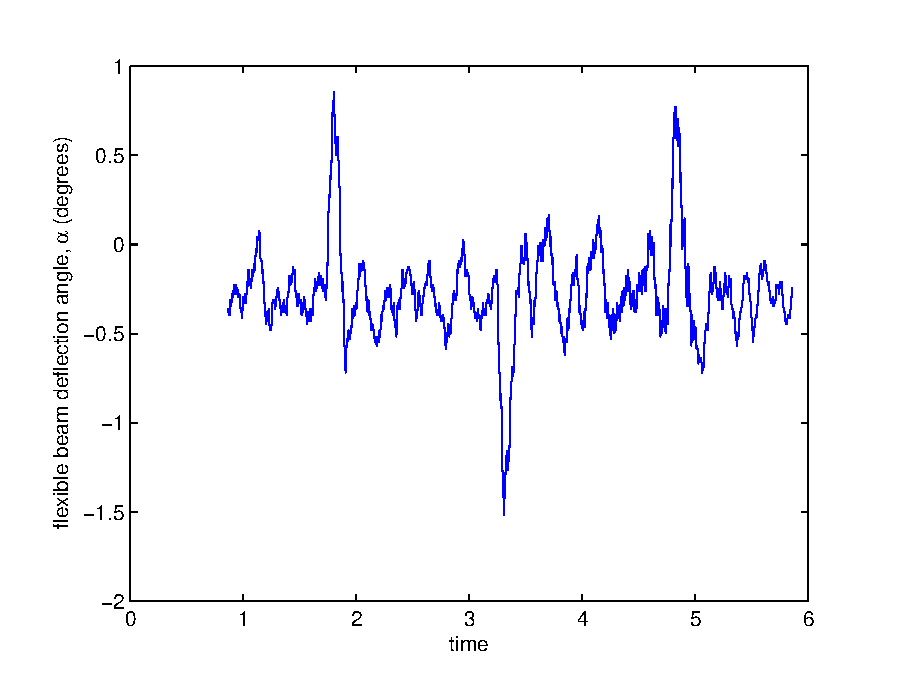
\includegraphics[width=0.5\linewidth]{eps/lab_4/alpha_q_1_1_1_1}}
                    %\caption{a) The rotor base response to a square wave input when $[q_1,\; q_2,\; q_3,\; q_4] = [1,\; 1,\; 1,\; 1]$, giving $[k_1,\; k_2,\; k_3,\; k_4] = [1,\; -9.5873,\; 0.6004,\; -0.4092]$, and b) the corresponding flexible beam deflection angle with respect to time.}
                    %\end{figure}
                    %\begin{figure}[htb!]
                    %\subfigure{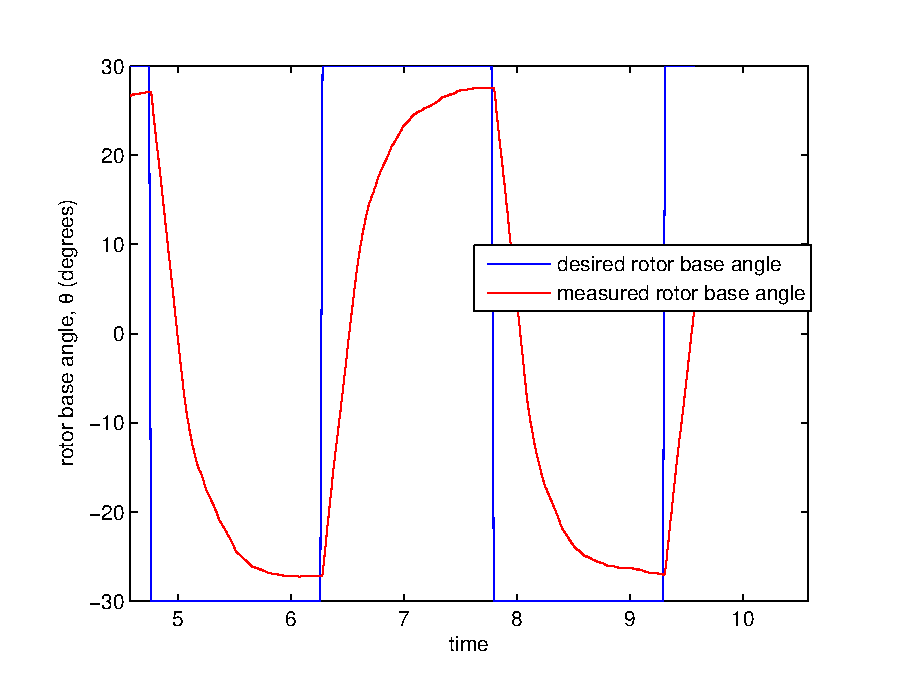
\includegraphics[width=0.5\linewidth]{eps/lab_4/theta_q_20_1_1_1}}
                    %\subfigure{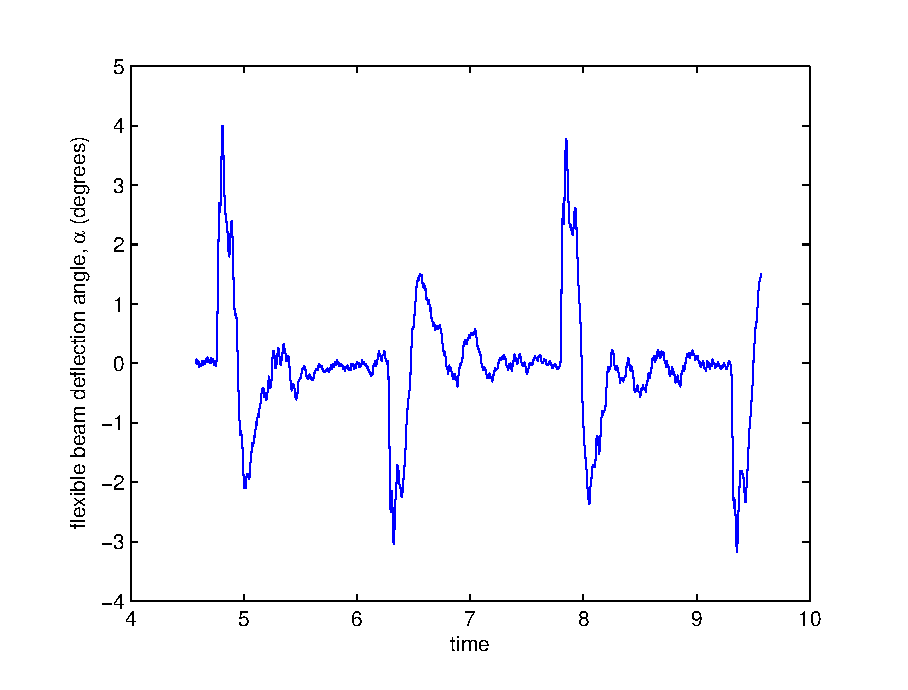
\includegraphics[width=0.5\linewidth]{eps/lab_4/alpha_q_20_1_1_1}}
                    %\caption{a) The rotor base response to a square wave input when $[q_1,\; q_2,\; q_3,\; q_4] = [20,\; 1,\; 1,\; 1]$, giving $[k_1,\; k_2,\; k_3,\; k_4] = [4.4721,\; -10.464,\; 0.798,\; -0.253]$, and b) the corresponding flexible beam deflection angle with respect to time.}
                    %\end{figure}
                    %\begin{figure}[htb!]
                    %\subfigure{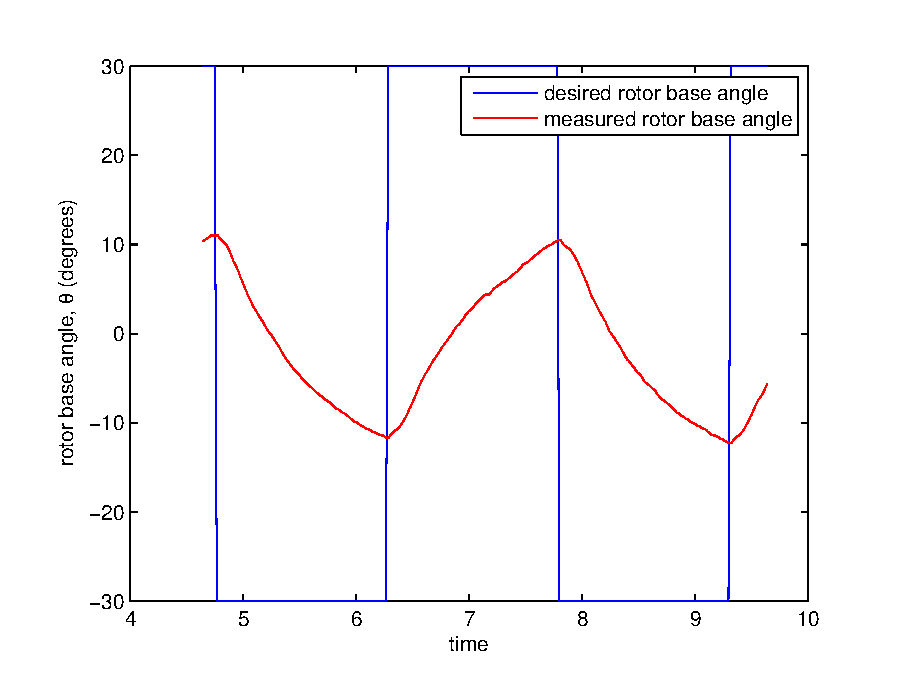
\includegraphics[width=0.5\linewidth]{eps/lab_4/theta_q_1_20_1_1}}
                    %\subfigure{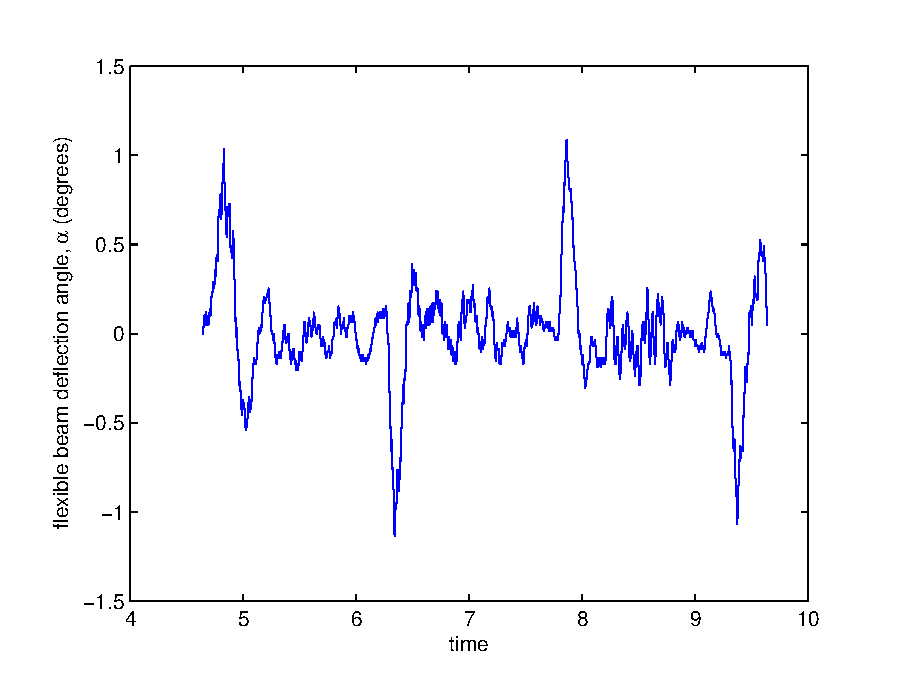
\includegraphics[width=0.5\linewidth]{eps/lab_4/alpha_q_1_20_1_1}}
                    %\caption{a) The rotor base response to a square wave input when $[q_1,\; q_2,\; q_3,\; q_4] = [1,\; 20,\; 1,\; 1]$, giving $[k_1,\; k_2,\; k_3,\; k_4] = [1,\; -10.408,\; 0.601,\; -0.413]$, and b) the corresponding flexible beam deflection angle with respect to time.}
                    %\end{figure}
                    %\begin{figure}[htb!]
                    %\subfigure{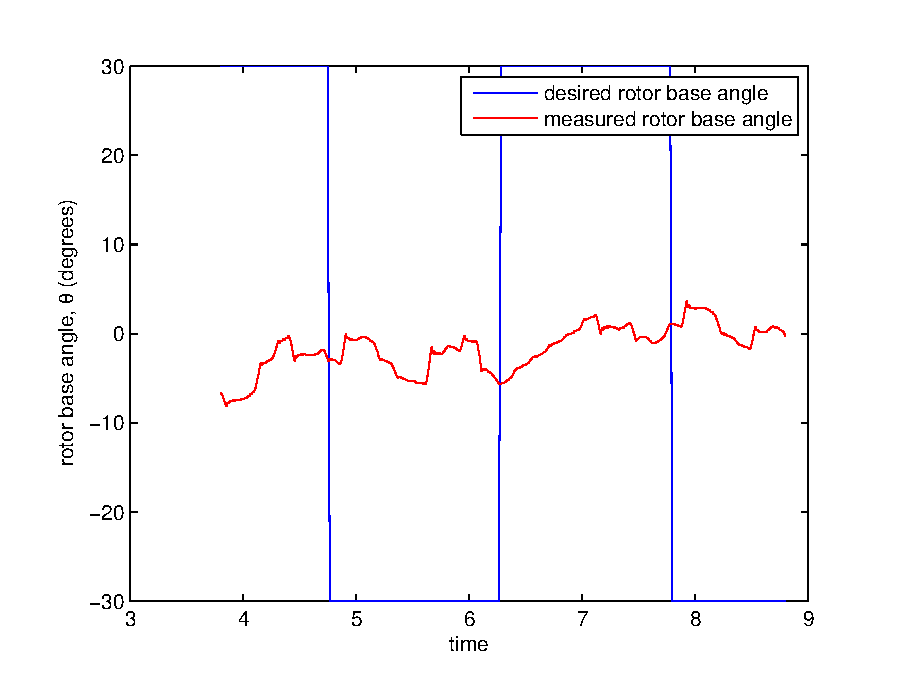
\includegraphics[width=0.5\linewidth]{eps/lab_4/theta_q_1_1_20_1}}
                    %\subfigure{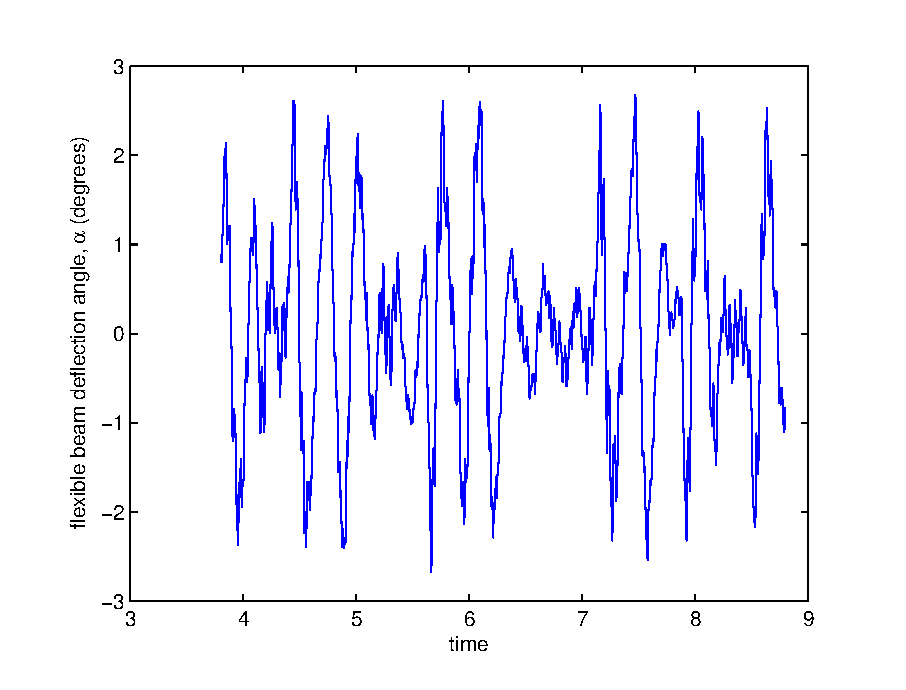
\includegraphics[width=0.5\linewidth]{eps/lab_4/alpha_q_1_1_20_1}}
                    %\caption{a) The rotor base response to a square wave input when $[q_1,\; q_2,\; q_3,\; q_4] = [1,\; 1,\; 20,\; 1]$, giving $[k_1,\; k_2,\; k_3,\; k_4] = [1,\; -10.85,\; 3.881,\; -0.133]$, and b) the corresponding flexible beam deflection angle with respect to time.}
                    %\end{figure}
                    %\begin{figure}[htb!]
                    %\subfigure{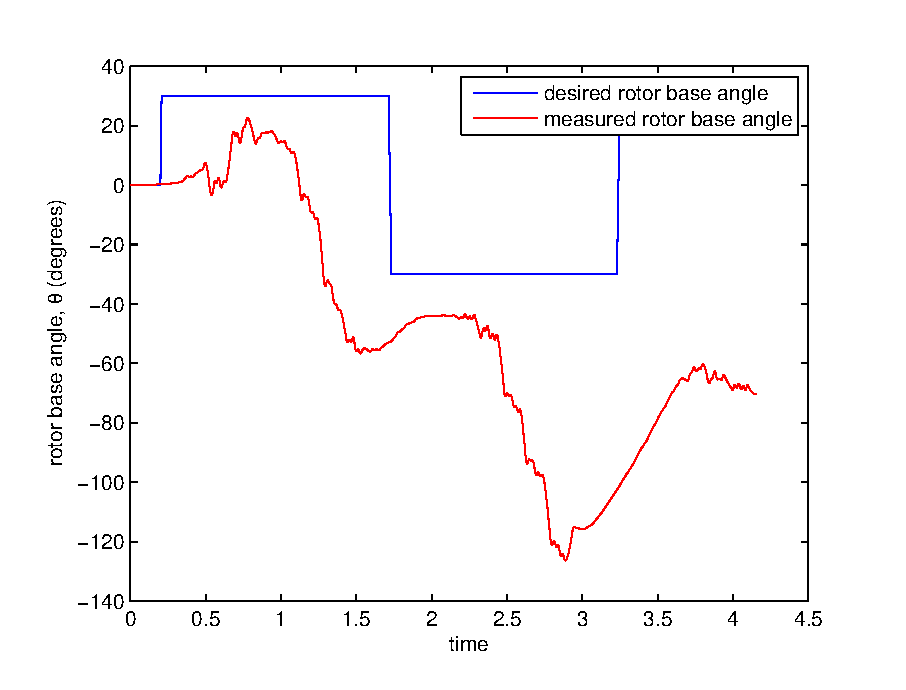
\includegraphics[width=0.5\linewidth]{eps/lab_4/theta_q_1_1_1_20}}
                    %\subfigure{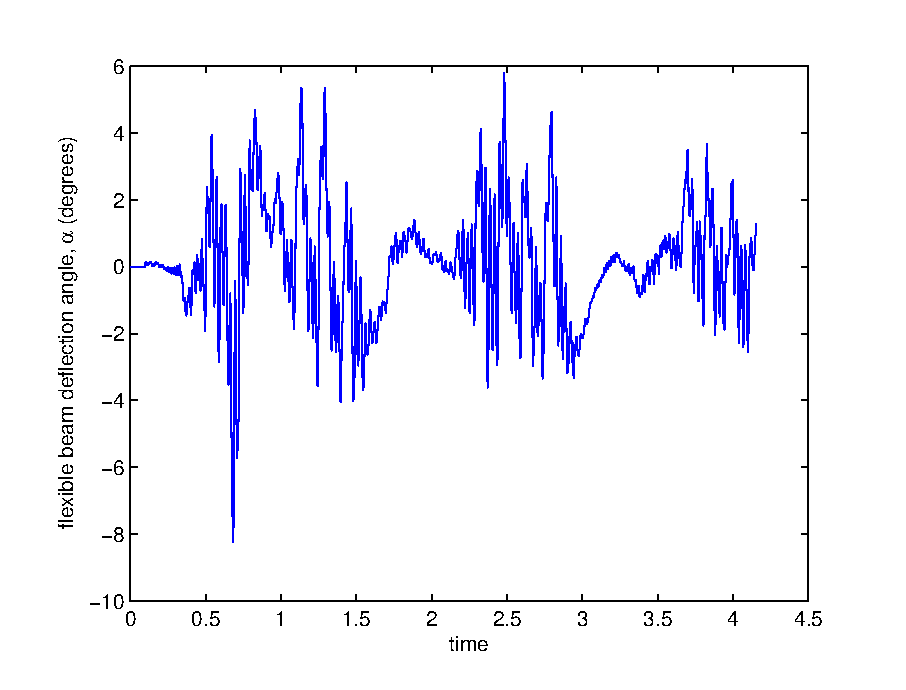
\includegraphics[width=0.5\linewidth]{eps/lab_4/alpha_q_1_1_1_20}}
                    %\caption{a) The rotor base response to a square wave input when $[q_1,\; q_2,\; q_3,\; q_4] = [1,\; 1,\; 1,\; 20]$, giving $[k_1,\; k_2,\; k_3,\; k_4] = [1,\; -43.48,\; 0.677,\; -3.449]$, and b) the corresponding flexible beam deflection angle with respect to time.}
                    %\end{figure}}

                    %\clearpage
                    %\drew{One will notice that increasing $q_1$ has an impact on changing $k_1$, and that the rotor base response is much faster (rise time and settling time is decreased). Also, increasing $q_4$ has a large impact on changing $k_4$, and thus from a theoretical standpoint, the angular velocity of the flexible beam should be reduced by increasing $q_4$. The other weightings, $q_2$ and $q_3$, have little effect on the system.
                    %}
              \item You will perform a similar experiment with the same input (square wave with amplitude of 30 and frequency of 0.33$Hz$), except now there are \emph{design restrictions} on the rotor base's response: we require that maximum percent overshoot to be 10\%, the rise time be within 0.5 seconds and the steady-state error be within 5\% for use in our application. In addition, the maximum flexible beam deflection should be no more than \(10^o\). Tune the diagonal weightings of $Q$ until you've achieved the desired results, and then plot the rotor's base angle, $\theta$, and the flexible beam's deflection angle, $\alpha$, with respect to time. Also plot the control input with respect to time. What weightings in the matrix $Q$ did you use to achieve these results, and what was the resulting feedback gain, $K$?
                    %\drew{Answer: The weightings that were used to achieve the desired performance was $[q_1,\; q_2,\; q_3,\; q_4] = [130,\; 1,\; 1,\; 3.5]$, giving $[k_1,\; k_2,\; k_3,\; k_4] = [11.401,\; -25.031,\; 1.379,\; -0.436]$. Instructors should note that there can be large variances between flexible beam modules, so these answers should be marked correct not by whether students can replicate the same weightings but by whether they can achieve that achieve the required response characteristics. Here are the plots:
                    %\begin{figure}[htb!]
                    %\center{
                    %\subfigure{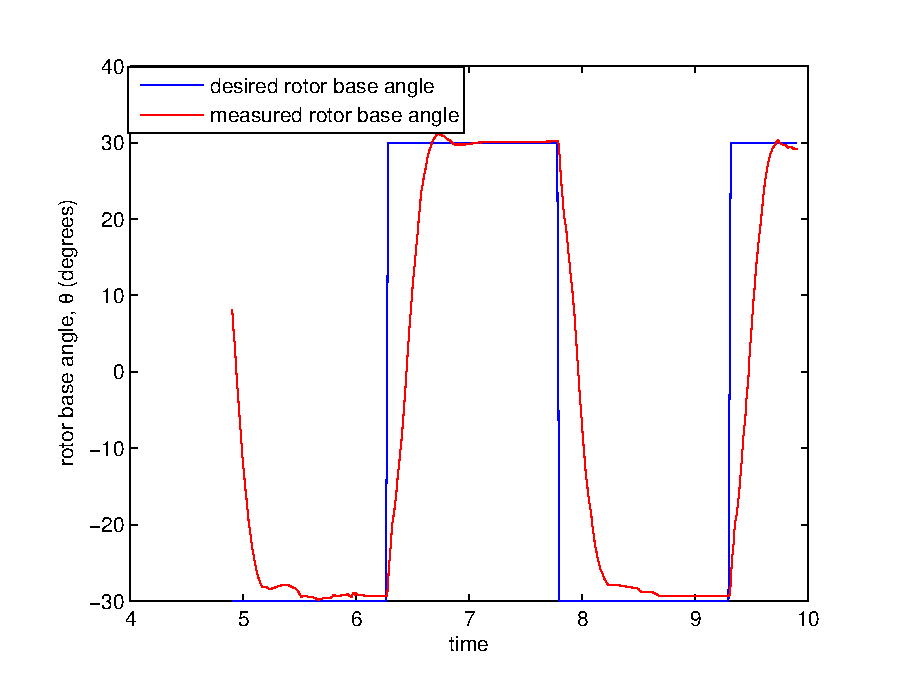
\includegraphics[width=0.4\linewidth]{eps/lab_4/theta_q_130_1_1_3half}}
                    %\subfigure{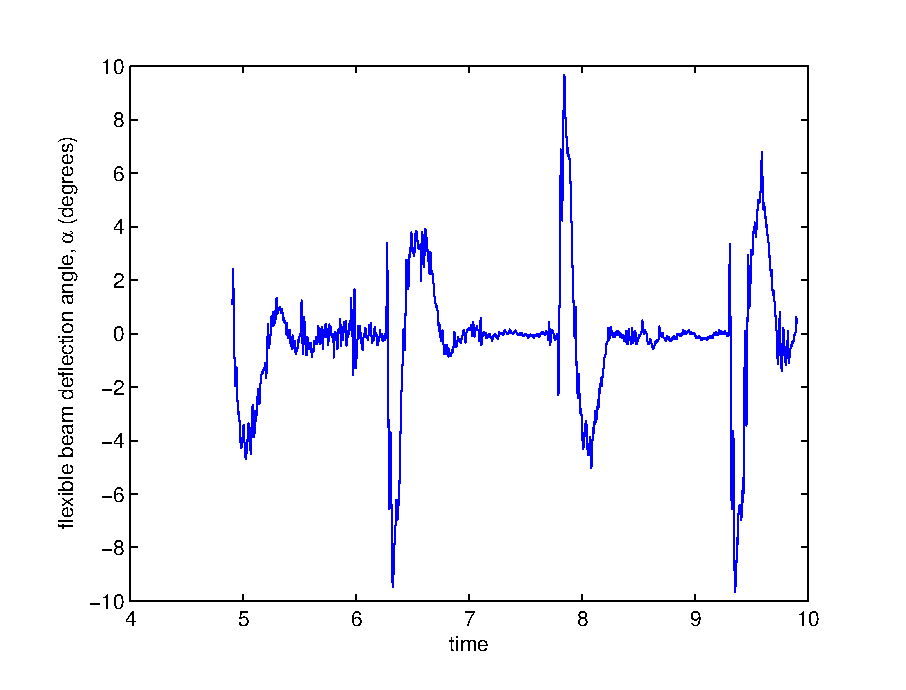
\includegraphics[width=0.4\linewidth]{eps/lab_4/alpha_q_130_1_1_3half}}
                    %\subfigure{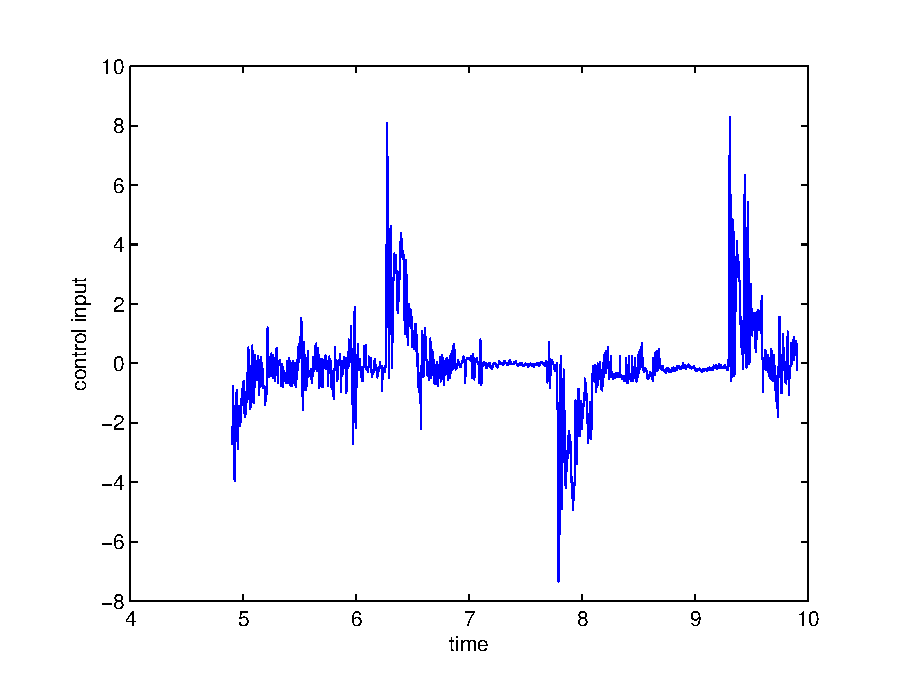
\includegraphics[width=0.4\linewidth]{eps/lab_4/vm_q_130_1_1_3half}}}
                    %\caption{a) The rotor base angle, and (b) the flexible beam deflection angle responses to a square wave input, with matrix $Q$ tuned to achieve the desired performance metrics.}
                    %\end{figure}
                    %}
          \end{enumerate}
    \item \textbf{Effects of Partial State Feedback on LQR}\label{subsection:lab4_partial_feedback}

          Now, you will observe the effects of using only partial state feedback in your closed-loop system on the optimality of the control system. Open the Simulink model \textbf{lqr\_partial\_feedback\_model.mdl}. Notice that the only state feedback being used is $\theta$ and the high-gain observer estimate of $\dot{\theta}$, as shown in Figure~\ref{lab4_lqr_partial_simulink}.
          \begin{figure}[htb!]
              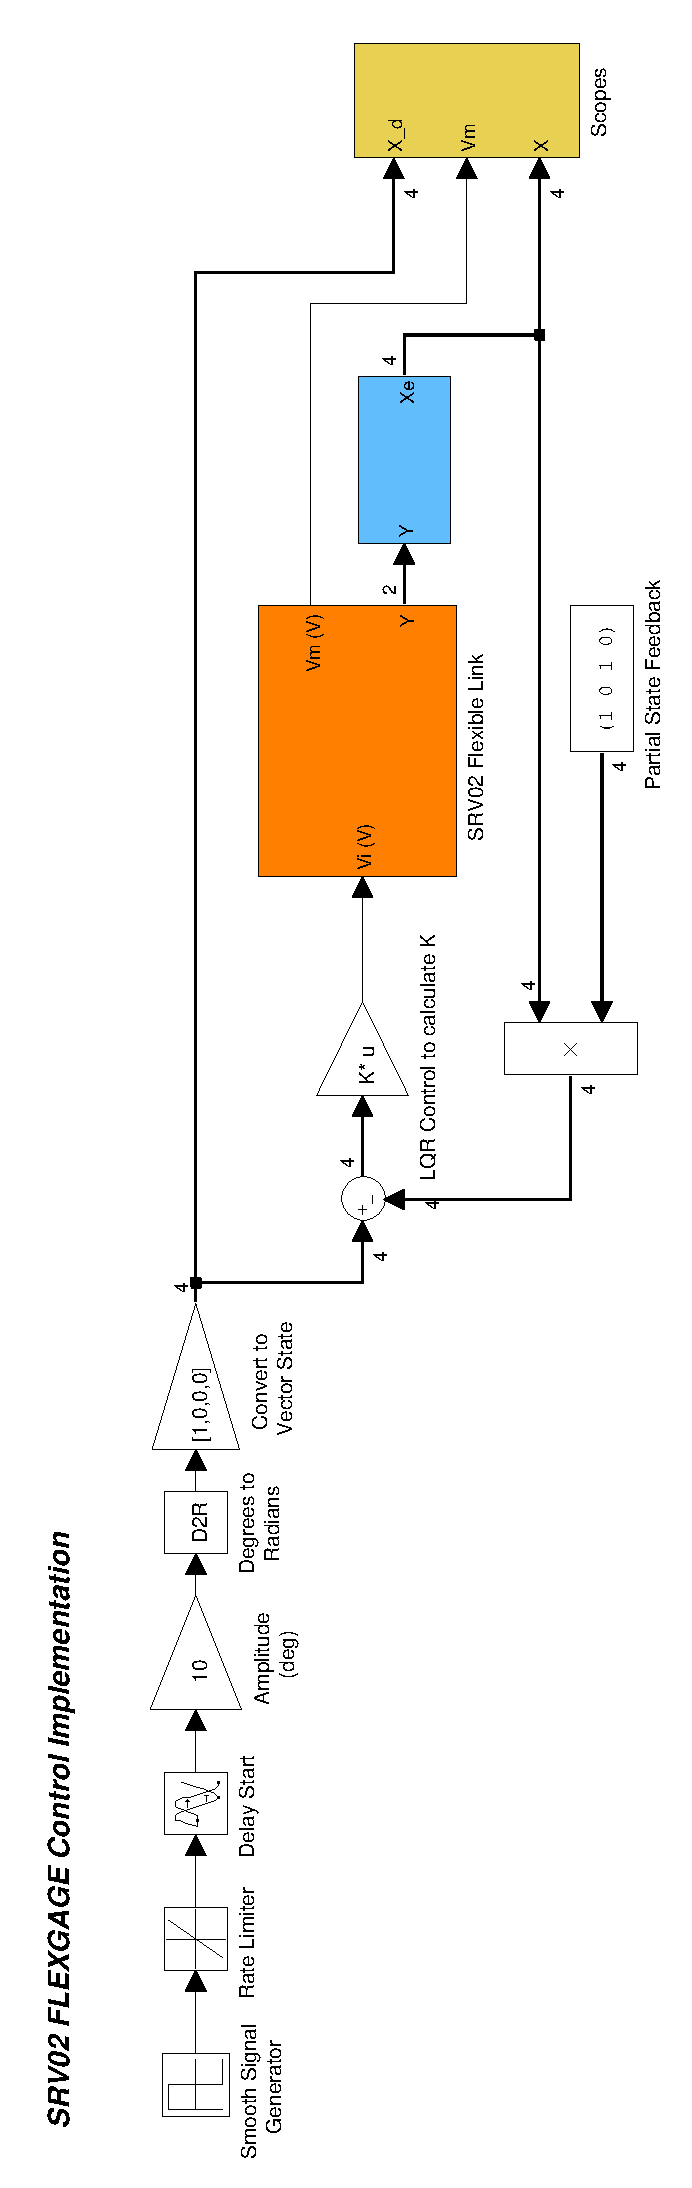
\includegraphics[width=0.3\linewidth,angle=-90]{eps/lab_4/lqr_partial_feedback_simulink}
              \caption{A Simulink model of the rotary flexible beam that utilizes partial state feedback and the linear quadratic regulator to design a feedback gain, $K$, that minimizes the deflections of the flexible beam while the rotor base tracks a square wave trajectory.}
              \label{lab4_lqr_partial_simulink}
          \end{figure}

          \begin{enumerate}
              \item Similar to the last experiment, use the LQR technique and the same weighting matrix $Q$ when computing your feedback gain, $K$. Plot the system responses to a square wave function with amplitude 30 and with frequency of 0.33 Hz. Compare the optimality of full state feedback and the partial state feedback closed-loop systems. Describe at least two previously-learned techniques that you may employ (and describe how) to obtain a better state feedback design, leading to superior system behaviour.
                    %\drew{Answer: in the partial state feedback case, the closed-loop control system is less optimal than the full state feedback system: the beam deflects much more and the steady-state error is higher. Due to the design of the cost function, these increases in beam deflection and steady-state error result in a higher cost. The control input is slightly less, but due to the design of the cost function, this will lower the cost significantly.
                    %\begin{figure}[htb!]
                    %\subfigure{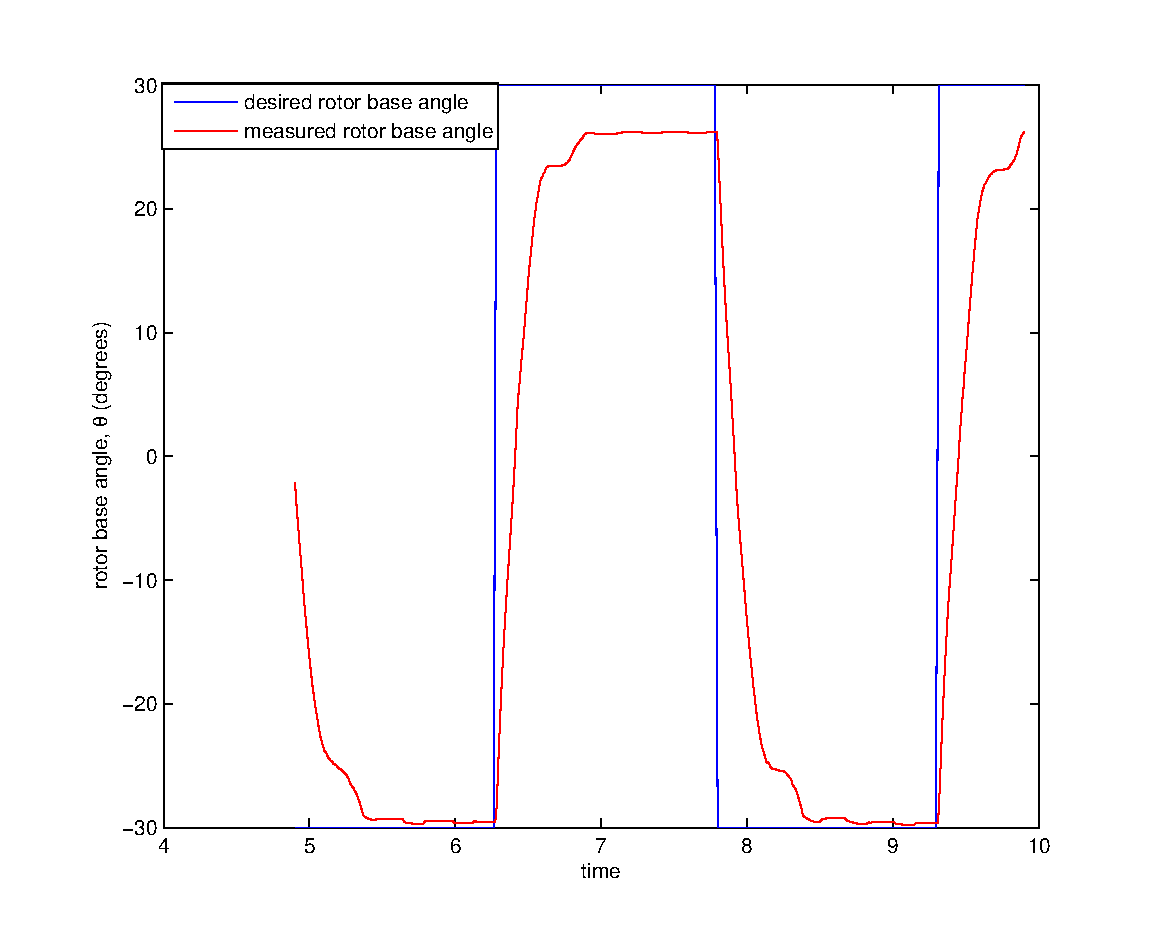
\includegraphics[width=0.48\linewidth]{eps/lab_4/theta_q_130_1_1_3half_partial}}
                    %\subfigure{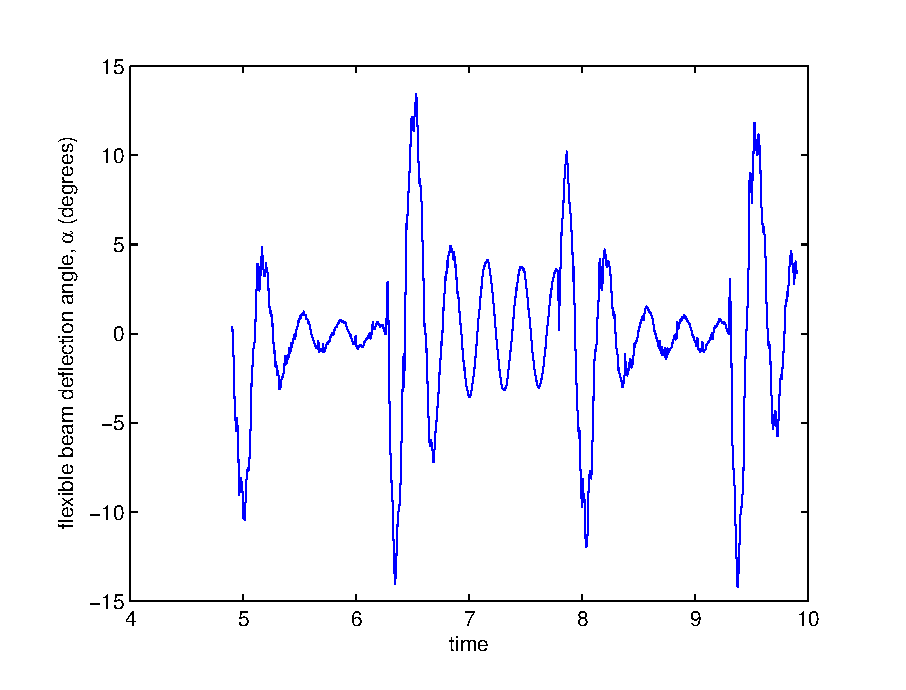
\includegraphics[width=0.5\linewidth]{eps/lab_4/alpha_q_130_1_1_3half_partial}}
                    %\center{
                    %\subfigure{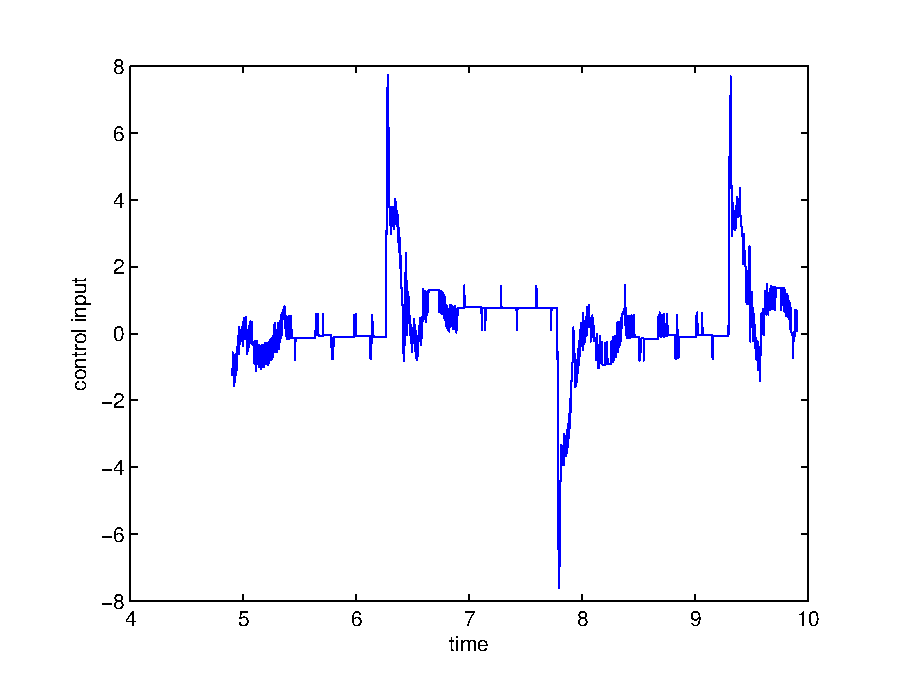
\includegraphics[width=0.5\linewidth]{eps/lab_4/vm_q_130_1_1_3half_partial}}}
                    %\caption{a) The rotor base angle, and (b) the flexible beam deflection angle responses to a square wave input when using only partial state feedback. This partial state feedback control system is less optimal than the full state feedback control system.}
                    %\end{figure}
                    %}
          \end{enumerate}

    \item \textbf{Designing an Observer \& Using Observer Estimate as Feedback for LQ Problem}\label{section:lab4_observer_lqr}
          \begin{enumerate}
              \item Is it possible to construct an observer for the rotary flexible link system, for the scenario where the strain gauge, which reads the flexible beam's deflection angle, is damaged?
                    %\drew{Answer: with this modification, the state-space matrix $C$ becomes
                    %\[
                    %C = \left[\begin{array}{c c c c}
                    %1 & 0 & 0 & 0\\
                    %0 & 0 & 0 & 0
                    %\end{array}\right]
                    %\]
                    %and the observability matrix becomes
                    %\[
                    %\mathcal{O}_{(A,C)} = \left[\begin{array}{c c c c}
                    %1 & 0 & 0 & 0\\
                    %0 & 0 & 0 & 0\\
                    %0 & 0 & 1 & 0\\
                    %0 & 0 & 0 & 0\\
                    %0 & 623.77 & -40.49 & 0\\
                    %0 & 0 & 0 & 0\\
                    %0 & -25257.84 & 1639.61 & 623.77\\
                    %0 & 0 & 0 & 0
                    %\end{array}\right]
                    %\]
                    %which has full rank. The controllability matrix does not change. Thus the modified system is controllable and observable, which implies that it is detectable and stabilizable. Hence, one can hope to construct an observer for the state $\alpha$, and then use the high-gain observer subsystem block to estimate $\dot{\alpha}$.}
          \end{enumerate}

          \begin{figure}[htb!]
              \centering
              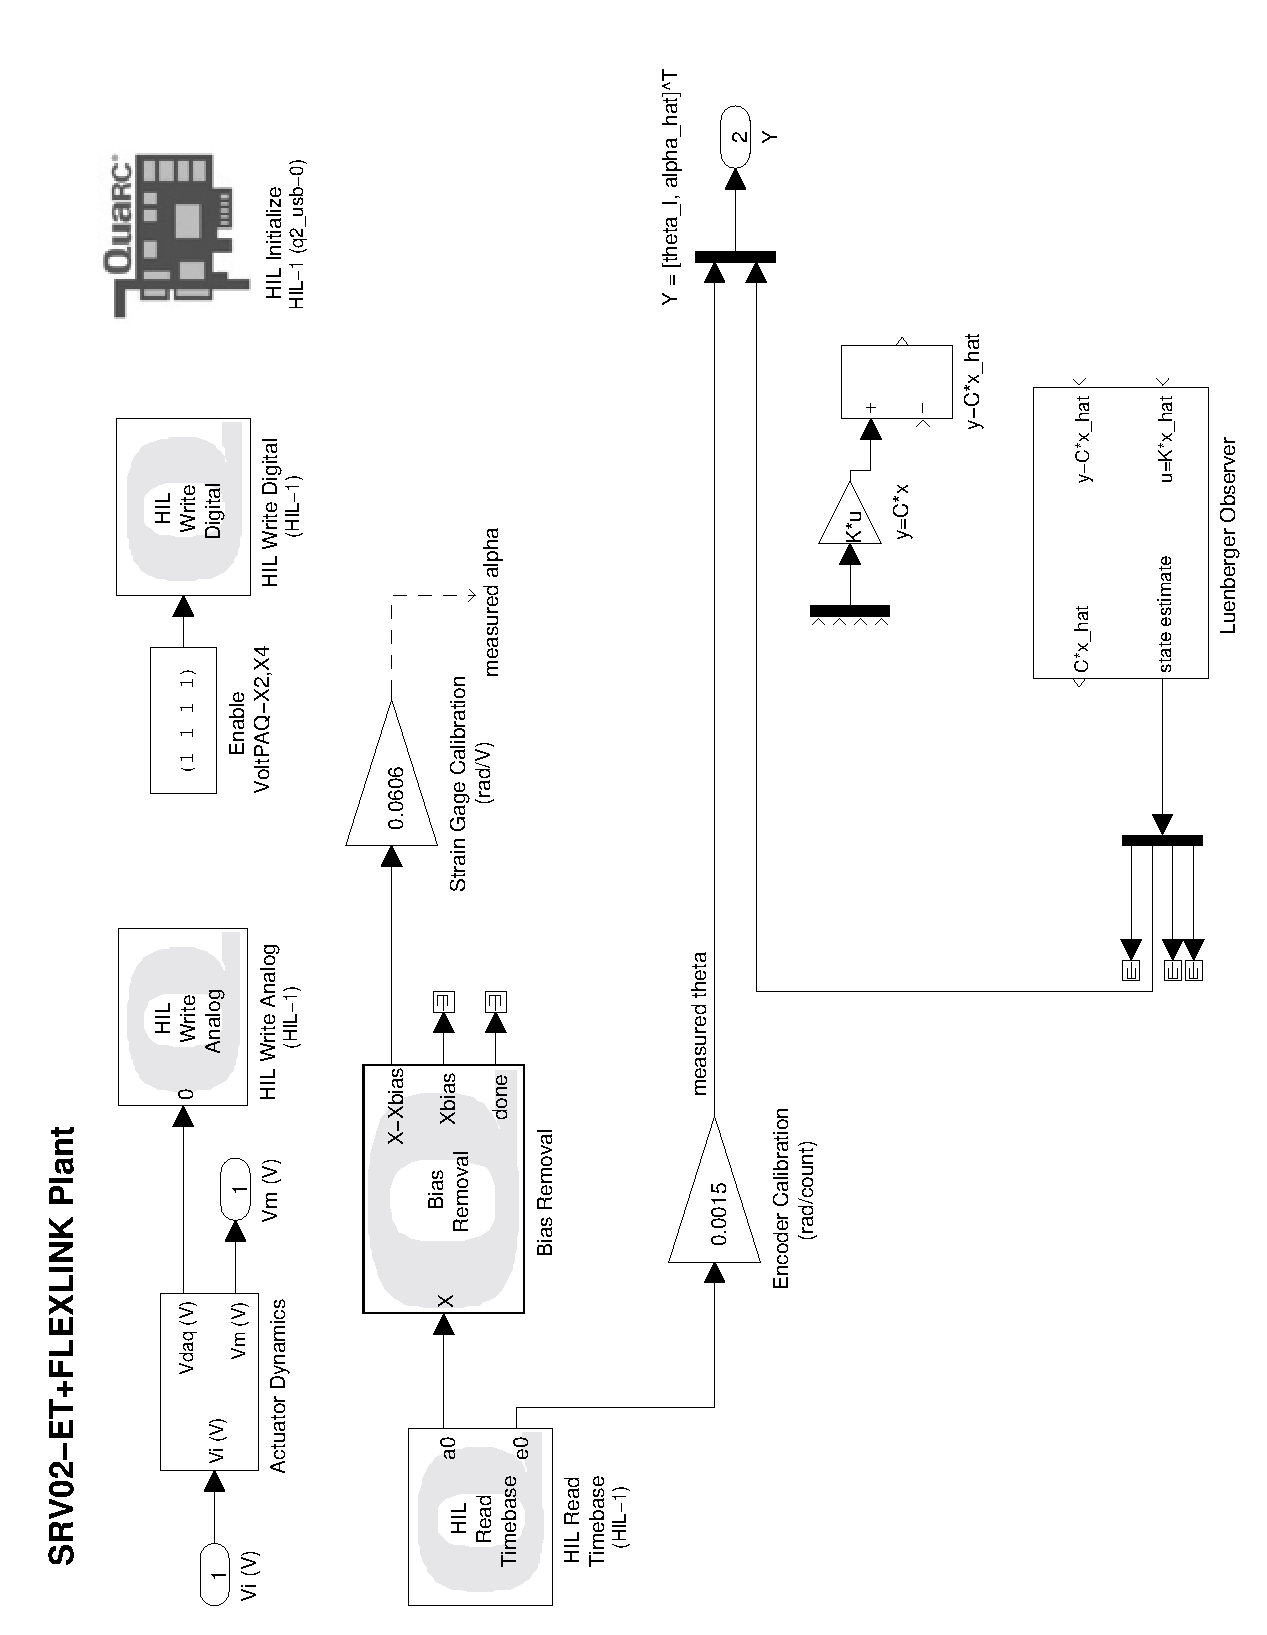
\includegraphics[width=0.6\linewidth,angle=-90]{eps/lab_4/lqr_observer_model}
              \caption{A Simulink subsystem block showing the rotary pendulum system and a Luenberger observer. These systems are not connected, however one can connect these in such a way to compare the measured and estimated pendulum angle, $\alpha$ and $\hat{\alpha}$, as well as use the pendulum angle estimate as LQR feedback. Note that this model will not run without modification.}
              \label{figure:lab4_lqr_observer_model}
          \end{figure}
          \newpage
          \begin{enumerate}
              \item Open the Simulink model \textbf{lqr\_observer\_model} with the Luenberger observer contained in the rotary pendulum's subsystem block, as shown in Figure~\ref{figure:lab4_lqr_observer_model}. Follow the procedure from Section~\ref{section:lab3_observer} of Lab 3 to build a Luenberger state observer to estimate state $\alpha$. You will need to tune your observer gain, $L$, similarly to how you did so in Lab 3 so that the observer dynamics are faster than the system dynamics. However, now your feedback gain $K$ is being produced by the linear quadratic regulator, so tuning $Q$ will alter $K$ and thus the observer gain $L$ may have to be tuned concurrently. \textbf{Make sure} to change your output matrix, $C$, such that $\alpha$ is not an output. Use the estimate of the beam's deflection angle, $\hat{\alpha}$, to calculate an estimate for the angular velocity of the beam via the high-gain observer subsystem. Plot the responses of the rotor base angle and the flexible beam deflection angle due to a square wave input of amplitude 30 and frequency 0.33Hz. On the flexible beam deflection angle plot, also plot your state estimate (you'll need to use a To Workspace block for this). What are your gains $L$ and $K$ and what is your weighting matrix $Q$? What can you conclude about the optimality (i.e., rotor base trajectory tracking and beam's deflections) of this control system when comparing it to the partial state feedback scenario and the full state feedback scenario?
                    %\drew{Answer: with $Q$ weightings of $[q_1,\; q_2,\; q_3,\; q_4] = [130,\; 1,\; 1,\; 3.5]$, the resulting feedback gain weightings are $[k_1,\; k_2,\; k_3,\; k_4] = [11.401,\; -25.031,\; 1.379,\; -0.436]$. The observer gain weightings are $[l_1,\; l_2,\; l_3,\; l_4] = [-40,\; -41,\; -42,\; -43]$. The plots below reveal that the state estimate, $\hat{\alpha}$, and $\alpha$ agree pretty well. As a result of using partial state feedback and state estimate feedback, the magnitude of the flexible beam deflections is reduced throughout in comparison to the partial state feedback closed-loop system. In comparison to the full state feedback system, the overall flexible beam deflections are greater, and the rotor angle response is almost the same. The control input for the state estimate feedback system is slightly less than that for the full state feedback system, although this decrease is only weighted by 1 in the cost function, whereas beam deflection is weighted by 3.5. Thus using the state estimates as feedback is a more optimal control system than using only partial feedback, but not as optimal as using full state feedback (as is expected).
                    %\begin{figure}[htb!]
                    %\subfigure{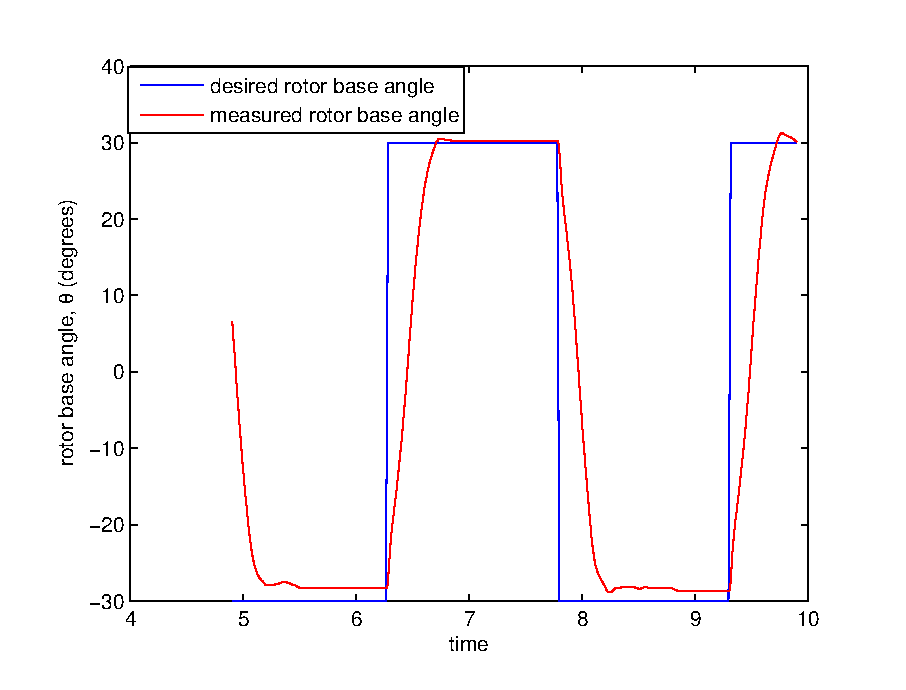
\includegraphics[width=0.5\linewidth]{eps/lab_4/theta_observer_feedback}}
                    %\subfigure{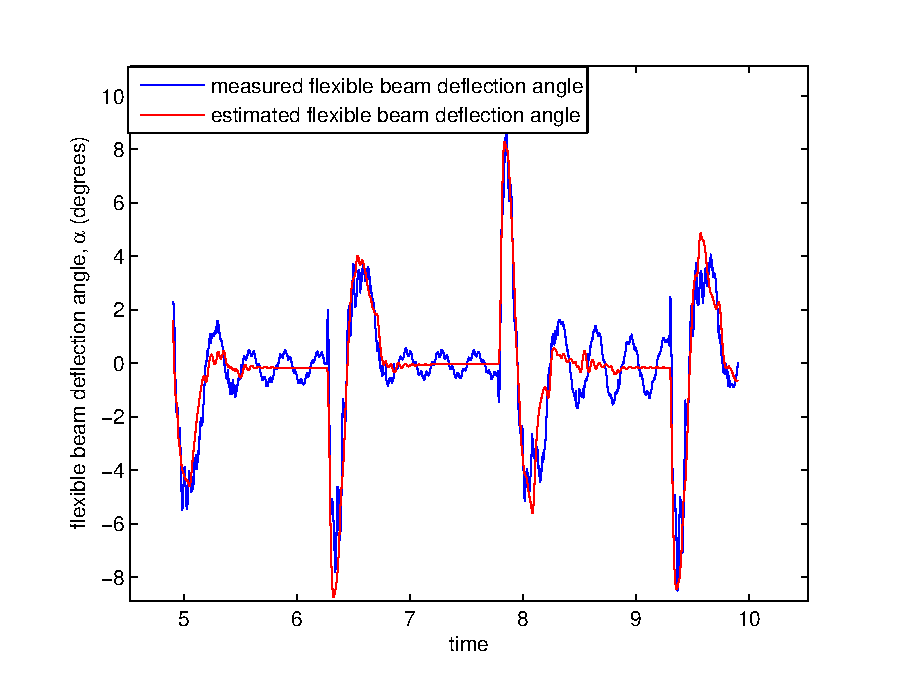
\includegraphics[width=0.5\linewidth]{eps/lab_4/alpha_observer_feedback}}
                    %\center{
                    %\subfigure{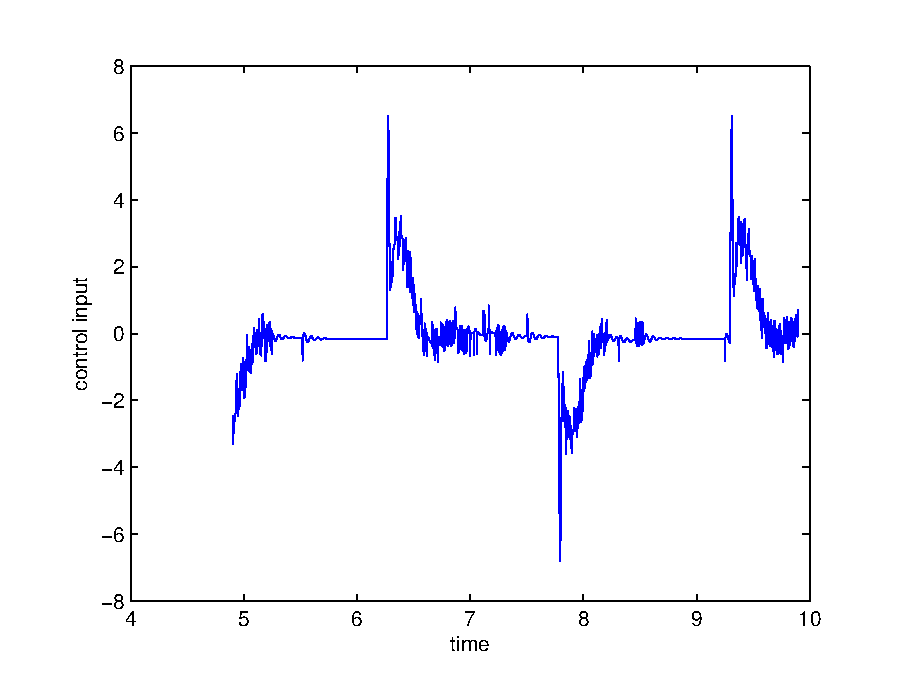
\includegraphics[width=0.5\linewidth]{eps/lab_4/vm_observer_feedback}}
                    %\caption{a) The rotor base angle, and (b) the flexible beam deflection angle responses to a square wave input when using partial state feedback $\theta$, $\dot{\theta}$ and state estimate feedback, $\hat{\alpha}$, $\hat{\dot{\alpha}}$. This control system is less optimal than the full state feedback control system, but more optimal than the partial state feedback system.}}
                    %\end{figure}
                    %}
          \end{enumerate}
\end{enumerate}

When you have completed the lab, make sure you save your files in a convenient location (e.g.\ on some type of cloud storage).

\section{Deliverables}
Prepare a brief write up describing what you learned from this lab. This does not need to be a formal report, but all material should be presented in a clear and logical manner, with concise descriptions where necessary. Include your answers to all the questions in the lab (these are the lettered sections in the procedure), as well as any requested plots.